\documentclass[beamer=true]{standalone}
\usepackage{preamblesnotes}

\begin{document}
\settitle{全內反射及應用\\Total internal reflection and application II}{光學第三課(II)}{周末班}





\begin{frame}{海市蜃樓Mirage}
\begin{figure}
    \centering
    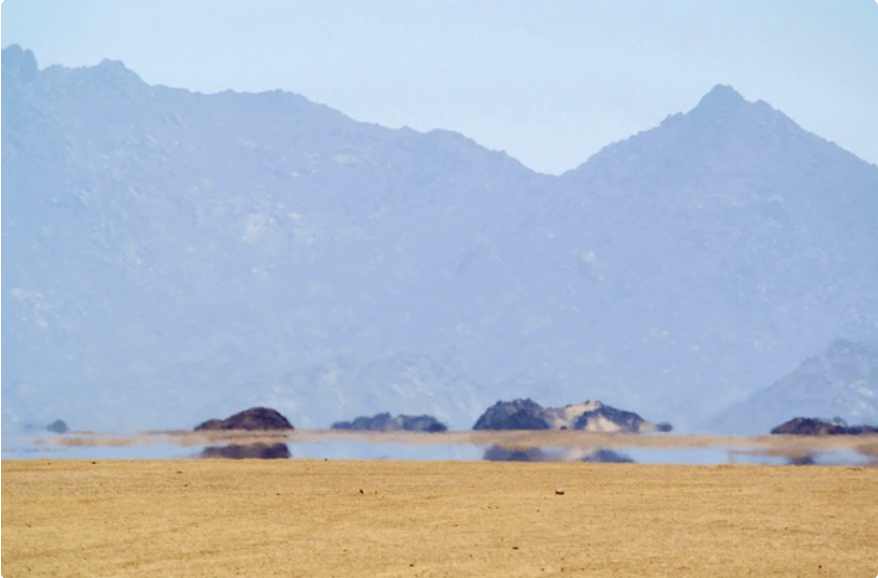
\includegraphics[width=0.5\linewidth]{assets/xue89nu98u8323.png}
\end{figure}
    \begin{figure}
        \centering
        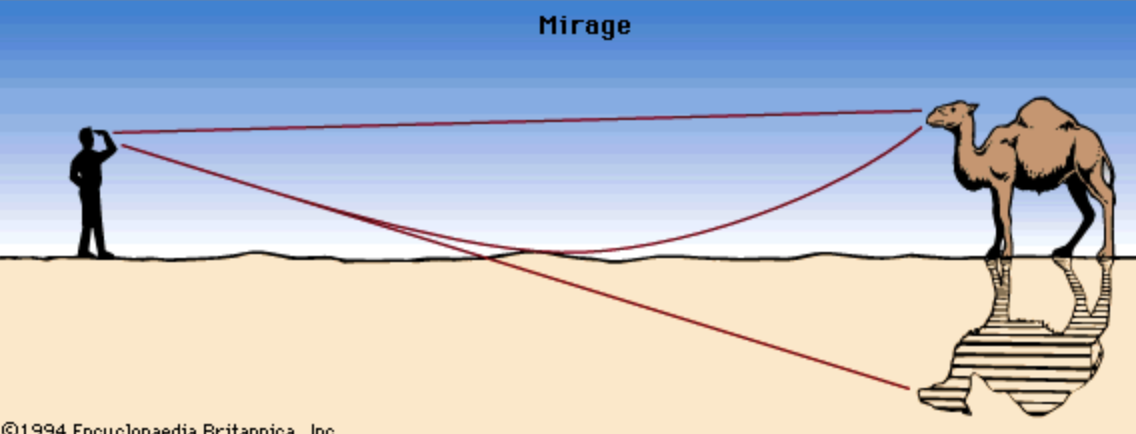
\includegraphics[width=0.75\linewidth]{assets/dm2u982und0un2389d3n209de.png}
        
        
    \end{figure}
      
\end{frame}

\begin{frame}{海市蜃樓Mirage}
\begin{itemize}
    \item 隨著高度的增加,溫度降低,光的速度減慢,空氣的折射率增加。\\As the height goes up, temperature goes down, speed of light decreases, refractive index of air increases.
    \item 光線在很長距離下持續徧離法線。\\Light rays bends away from normal continuously over long path length.
    \item 遠處地面上方的物體和空氣出現在地面上,使其看起來像水一樣。\\The objects above distant ground and the air appears on the ground, making it look like water.
    \item 在觀察者看來,由於光線來自相同入射角的遠處物體,所以海市蜃樓總是看起來在前方相同的距離。\\The mirage always seems to be at the same distance for an observer at similar places since the light rays are from distant object at the same incident angle.
\end{itemize}
    
\end{frame}



\begin{frame}{海市蜃樓(南/北極) Mirage (North/South pole)}
    \begin{figure}
        \centering
        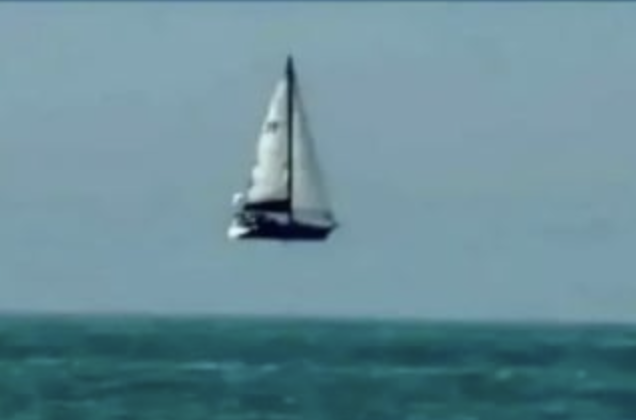
\includegraphics[width=0.5\linewidth]{assets/dijhheu32.png}
        
        
    \end{figure}
    \begin{figure}
        \centering
        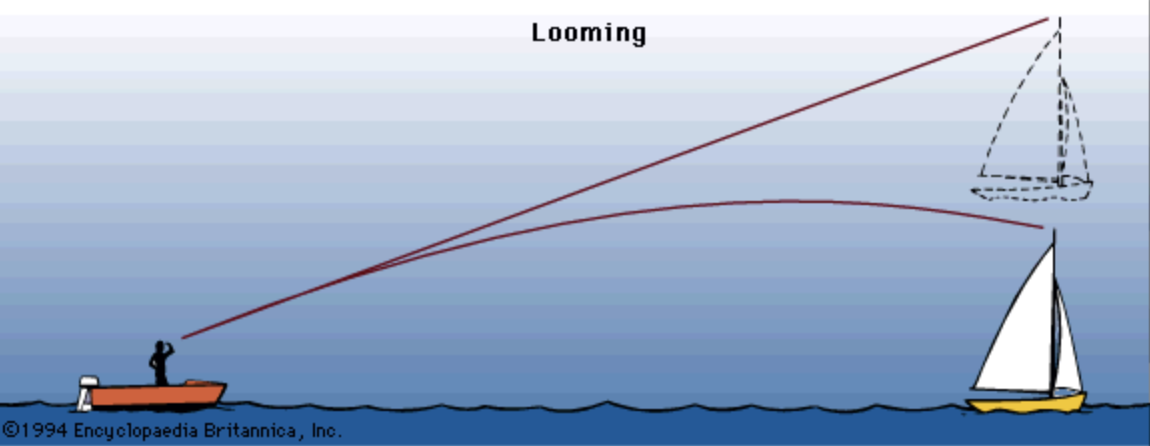
\includegraphics[width=0.75\linewidth]{assets/89xu0n908u12r.png}
        
        
    \end{figure}
\end{frame}
\begin{frame}{海市蜃樓(南/北極) Mirage (North/South pole)}
    \begin{itemize}
        \item 隨著高度的增加,溫度增加,光速增加,光線在空氣中的折射率下降。\\As height goes up, the temperature increases, speed of light increases, refractive index of air decreases.
        \item 光線在很長距離下持續偏向法線。\\Light rays continuously bends towards the normal over long path length.
        \item 船只看起來在天空中。\\The ship appears in the air.
        
    \end{itemize}

\end{frame}

\begin{frame}{海市蜃樓(南/北極) Mirage (North/South pole)}
\begin{itemize}
    \item 透過多次的折射和全內反射,令太陽升起的時間比它實際上的時間早,或是日落時太陽落下得比它實際上的時間晚\\Through multiple refractions and total internal reflections, the sunrise appears to occur earlier than its actual time, or the sunset appears to happen later than its actual time.
\end{itemize}
    \begin{figure}
        \centering
        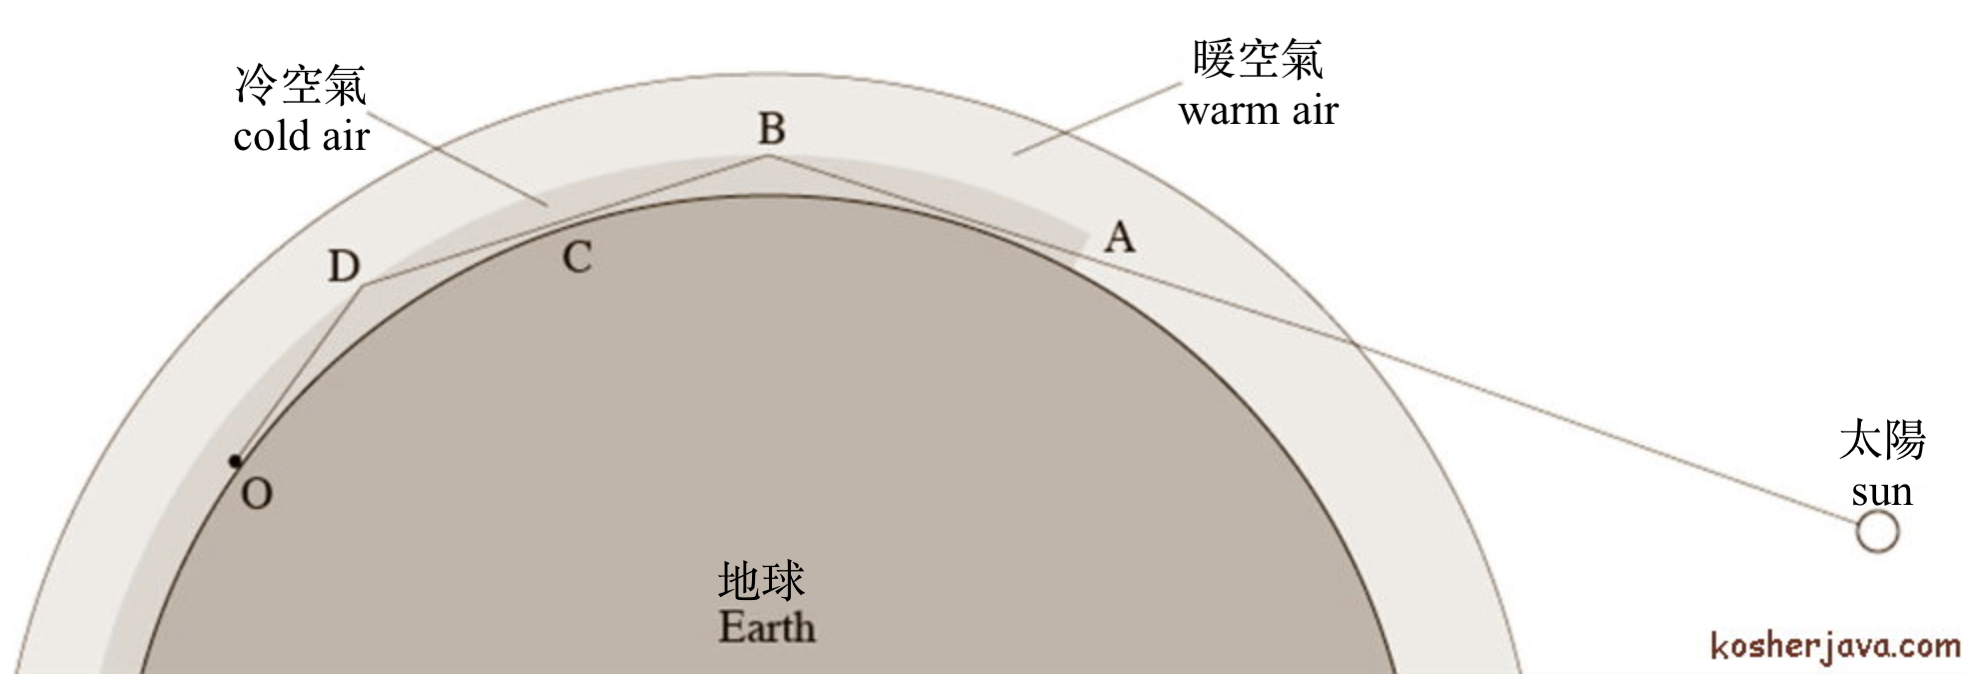
\includegraphics[width=1\linewidth]{assets/deijoii23jnd2398fy98.png}
    \end{figure}
\end{frame}

\begin{frame}{三稜鏡的全內反射Total reflecting prism}
    \begin{itemize}
        \item 對於玻璃棱鏡來說,光的折射率為1.5。\\For glass prism, refractive index is 1.5.
        \item 臨界角Critical angle $\theta_c=$
        \item 如果玻璃內的入射角大於臨界角,就會發生全內反射。所有光的強度都被完全反射。\\If the incident angle inside the glass is greater than this critical angle, total internal reflection occurs. All the intensity of the light is totally internal reflected.
    \end{itemize}
    \begin{figure}
        \centering
        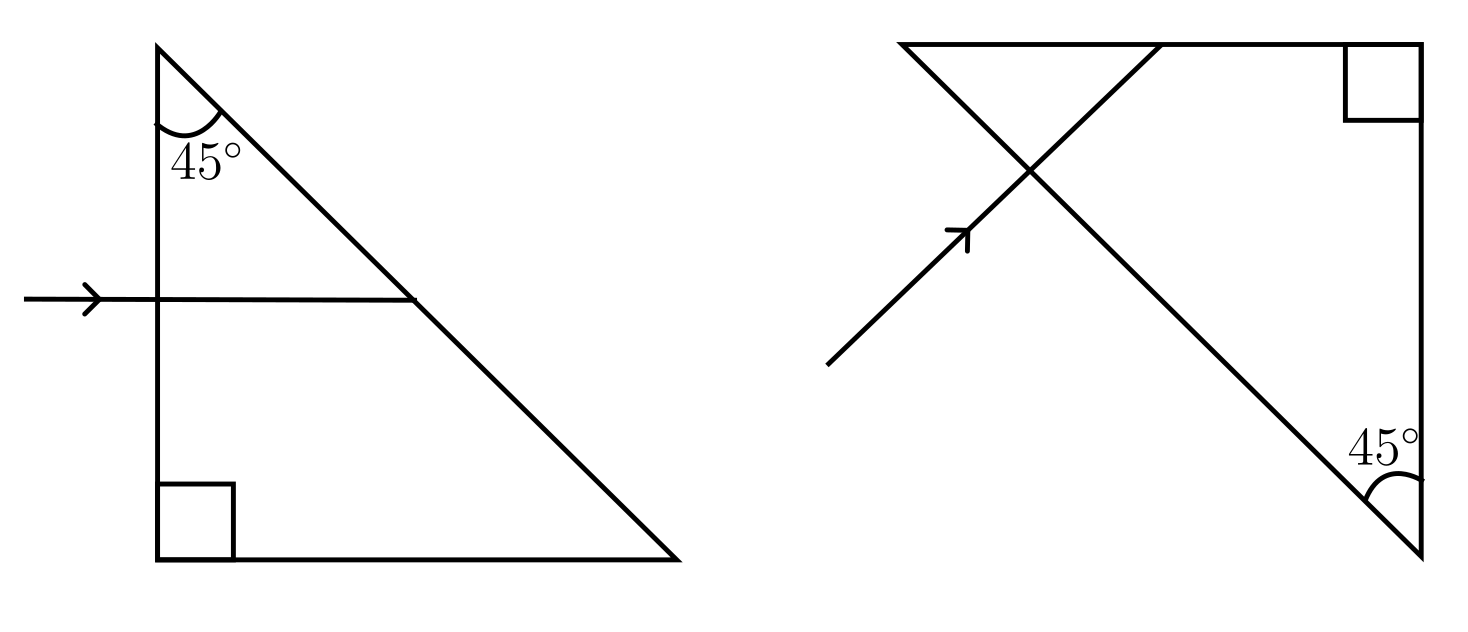
\includegraphics[width=0.55\linewidth]{assets/dmdnuu.png}
    \end{figure}
\end{frame}

\begin{frame}{望遠鏡Binoculars}
    \begin{itemize}
        \item 雙筒望遠鏡通常會在其中加入棱鏡,來減少望遠鏡的長度並達到更大的最大放大倍率。\\Prisms are often added in binoculars to reduce the length of the binocular and achieve greater maximum magnification.
    \end{itemize}
    \begin{figure}
        \centering
        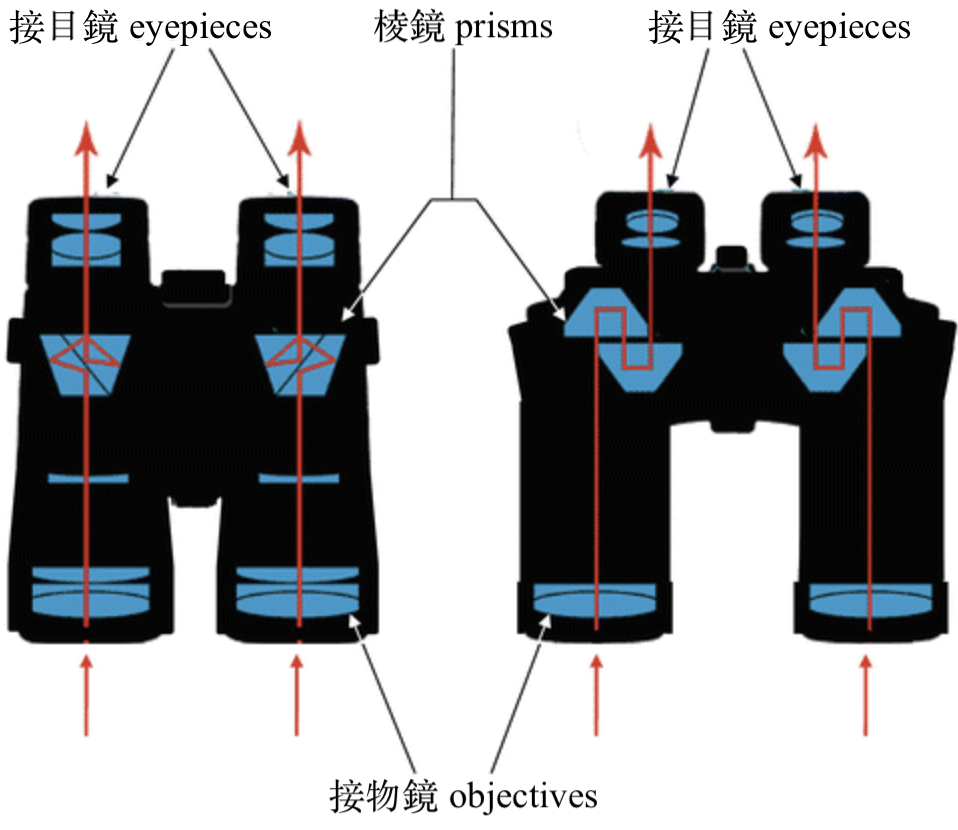
\includegraphics[width=0.58\linewidth]{assets/dun892u983n928dn82u3c.png}
        
        
    \end{figure}
\end{frame}

\begin{frame}{潛望鏡Periscopes}
\begin{itemize}
    \item 稜鏡來製作潛望鏡相較於平面鏡的優勢:\\The advantages of using a prism to make a periscope compared to a flat mirror are as follows:
    \begin{itemize}
        \item 沒有多重反射發生。\\No multiple reflection occurs.
        \item 成像將會更光亮和更清晰。\\The image will be brighter and clearer.
    \end{itemize}
\end{itemize}
    \begin{figure}
        \centering
        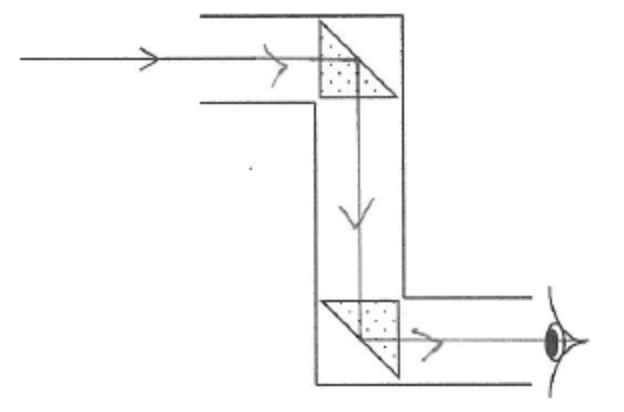
\includegraphics[width=0.5\linewidth]{assets/dqwdjmd9n0d98329bdy872yd.png}
    \end{figure}
\end{frame}

\begin{frame}{鑽石Diamonds}
\begin{itemize}
    \item 鑽石的折射率非常高,因此臨界角很小。因此全內反射很容易發生。\\Diamond has a very large refractive index, thus the critical angle is small. Therefore, total internal reflection would occur easily.
    \begin{itemize}
        \item $\therefore$鑽石看起來比玻璃更閃爍。\\$\therefore$ Real diamonds looks more sparkling than glass diamonds.
    \end{itemize}
\end{itemize}
\begin{figure}
    \centering
    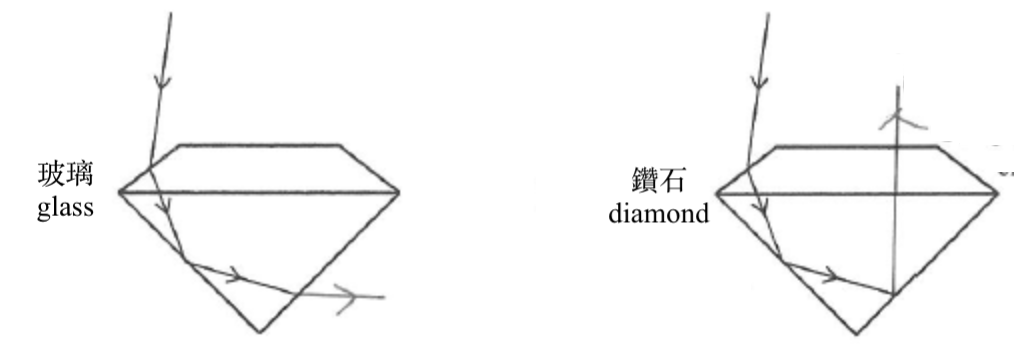
\includegraphics[width=0.75\linewidth]{assets/snu892u98du2d982.png}
    
    
\end{figure}

\end{frame}

\begin{frame}{鑽石Diamonds}
\begin{itemize}
    \item 鑽石被切割成特別的形狀,以便大部分進入鑽石的光線能夠被全內反射並傳遞到上方,使其看起來非常閃爍。\\Diamond should be cut so that most of the light entering the diamond would be total internal reflected and transmitted above so that it seems to be very sparkling.
\end{itemize}
    \begin{figure}
        \centering
        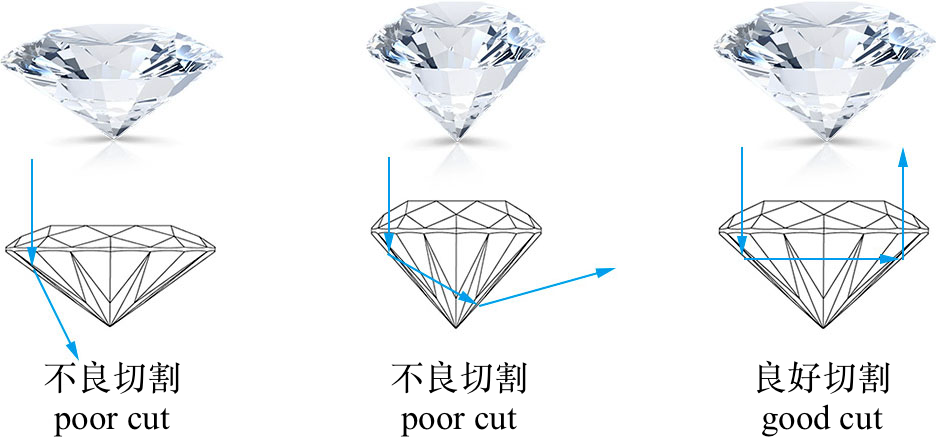
\includegraphics[width=0.8\linewidth]{assets/d8n9xudn8392dfr.png}
        
        
    \end{figure}
\end{frame}

\begin{frame}{光纖Optical fibers}
\begin{figure}
    \centering
    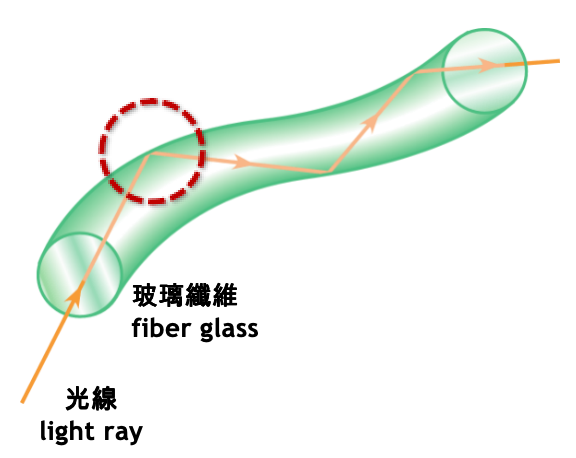
\includegraphics[width=0.4\linewidth]{assets/dj893d8239823age.png}
    
    
\end{figure}
    \begin{figure}
        \centering
        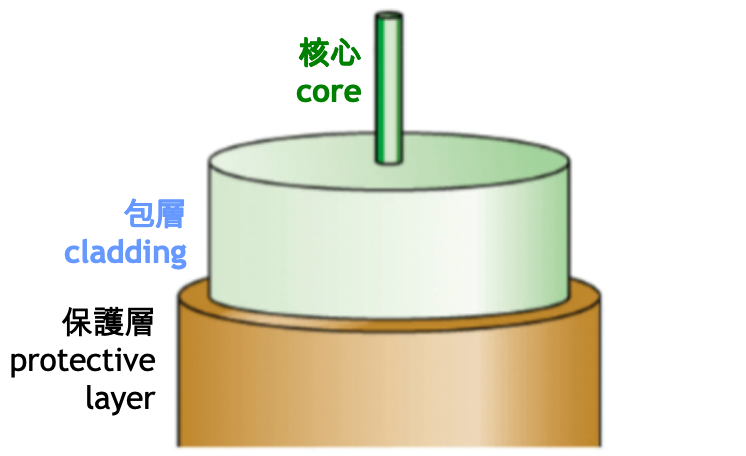
\includegraphics[width=0.4\linewidth]{assets/ddj32e.png}
        
        
    \end{figure}
\end{frame}




\begin{frame}{光纖的應用Application of optical fibers}
    \begin{figure}
    \centering
    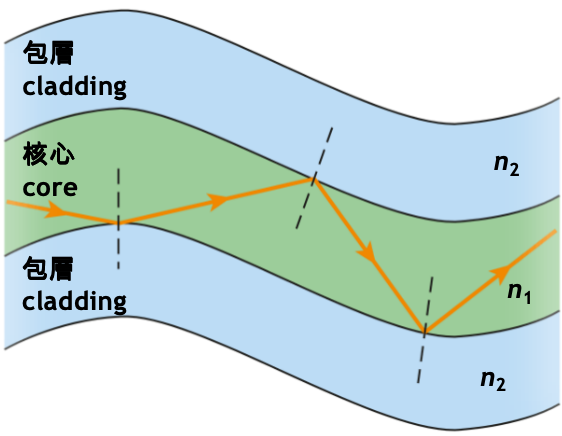
\includegraphics[width=0.4\linewidth]{assets/32e23d234f5.png}
\end{figure}
\begin{figure}
    \centering
    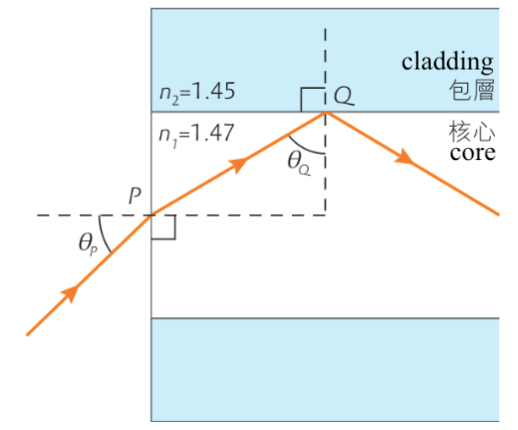
\includegraphics[width=0.4\linewidth]{assets/djnu349bd9843fge.png}
\end{figure}
\end{frame}

\begin{frame}{光纖的應用Application of optical fibers}
\begin{itemize}
    \item $n_2<n_1$:
    \begin{itemize}
        \item 使核心中的光線能發生全內反射。\\To make total internal reflection occur between boundaries for light inside the core.
    \end{itemize}
    \item $n_2\approx n_1$ 和and $n_2<n_1$:
    \begin{itemize}
        \item 臨界角 critical angle $=\sin^{-1}\left(n_2/n_1\right)$
        \item 使大入射角進入光纖的光線在包層折射出去,令接收到的光脈衝寛度減少,訊號更集中。\\The light rays entering the optical fiber at large incident angles are refracted out by the cladding, resulting in reduced pulse broadening and more focused signal reception.
    \end{itemize}
\end{itemize}
\end{frame}

\begin{eg}
    一條光線入射在一條光纖核心上的P點,然後,在核心的Q點發 生全內反射。已知光纖的核心和包層兩者的折射率分別為1.47和 1.45。\\A light ray enters the core of a straight optical fiber from air at position P as shown. It is then totally reflected at position Q. The core and the cladding have refractive indices of 1.47 and 1.45, respectively.
    \begin{figure}
    \centering
    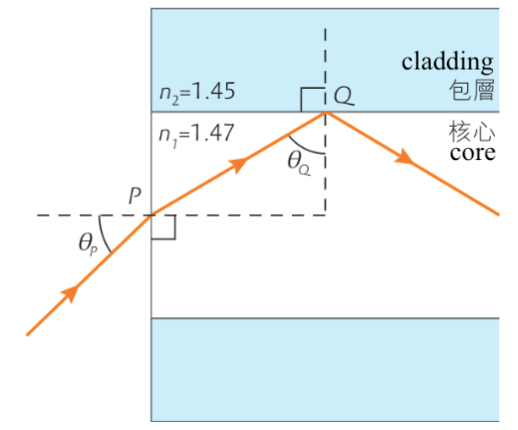
\includegraphics[width=0.5\linewidth]{assets/djnu349bd9843fge.png}
\end{figure}
\end{eg}

\begin{eg}
    \begin{itemize}
        \item [(a)] 若要在 Q 點發生全內反射,	在 P 點的入射角最大可為多少?\\What is the maximum angle of incidence at P so that total internal reflection occurs at Q?
    \end{itemize}

\end{eg}

\begin{eg}
    \begin{itemize}
        \item [(b)] 已知光纖全長 2 km,光線從一端傳播至另一端所需的時間最長為多久?\\The fiber is 2 km long. Find the longest time for light to travel from one end to the other.
    \end{itemize}

\end{eg}

\begin{eg}
    \begin{itemize}
        \item [(c)] 倘若核心的折射率稍微上升,則 (b) 部的答案如何改變?\\The refractive index of the core is now slightly higher. How does the time in (b) change?
    \end{itemize}
    
\end{eg}

\begin{frame}{光纖用於通訊Optical fiber for telecommunications}
    \begin{figure}
        \centering
        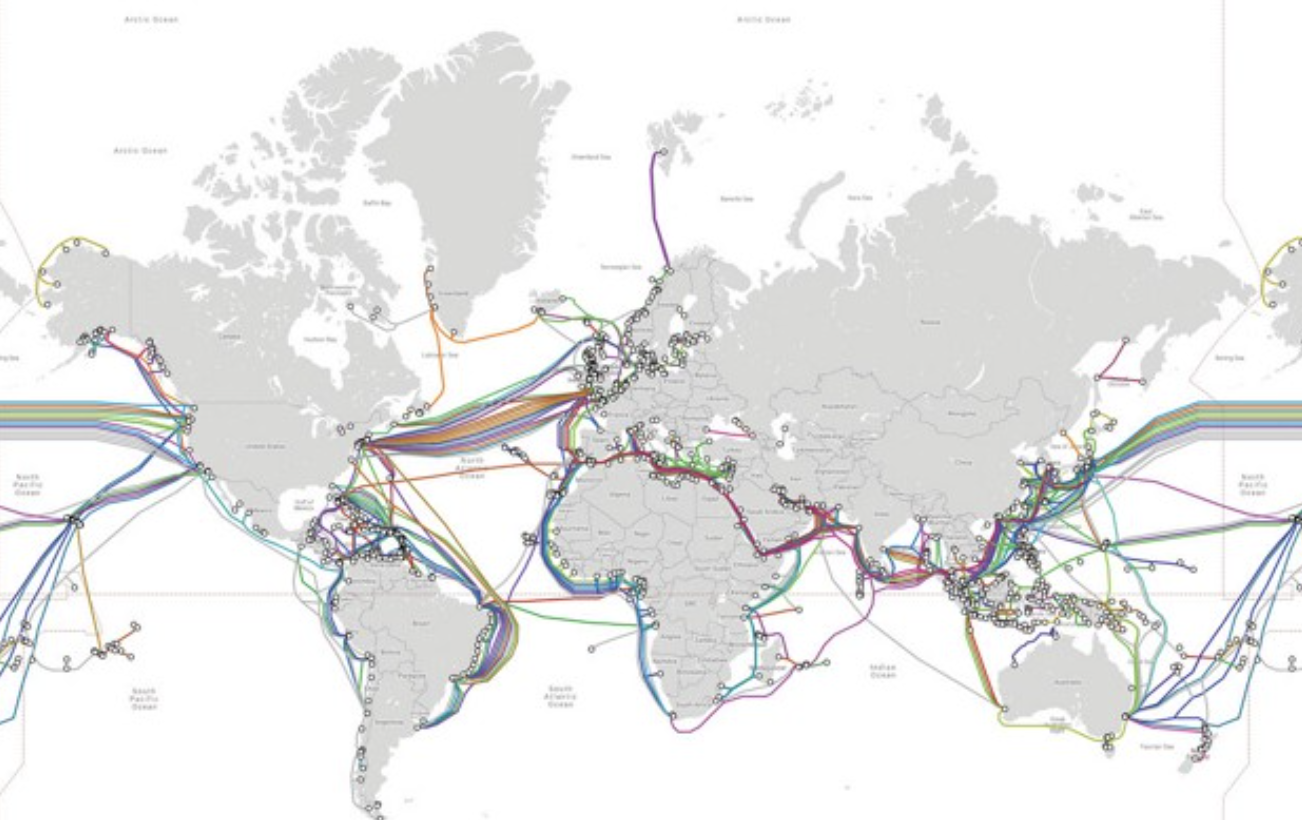
\includegraphics[width=0.75\linewidth]{assets/dqwd120d.png}
        \caption{海底光纖電纜組成的網絡在全球交叉穿梭,承載著全球的電信信號。A network of undersea fiber-optic cables crisscrosses the globe, carrying the world's telecommunication signals.}
        
    \end{figure}
    
\end{frame}

\begin{frame}{光纖用於通訊Optical fiber for telecommunications}
    \begin{itemize}
        \item 使用光纖電纜相較於銅電纜在電信上的優勢:\\Advantages of using optical fiber cables over copper cables for telecommunication:
        \begin{itemize}
            \item 光纖能夠以極少的能量損耗傳輸信號。\\Optical fibers transmit signals with little loss of energy.
            \item 光纖能夠承載更多的資訊。\\Optical fibers can carry more information.
            \item 光纖更輕巧且更纖細。\\Optical fibers are lighter and thinner.
        \end{itemize}
    \end{itemize}
\end{frame}

\begin{frame}{內窺鏡Endoscope}
    \begin{figure}
        \centering
        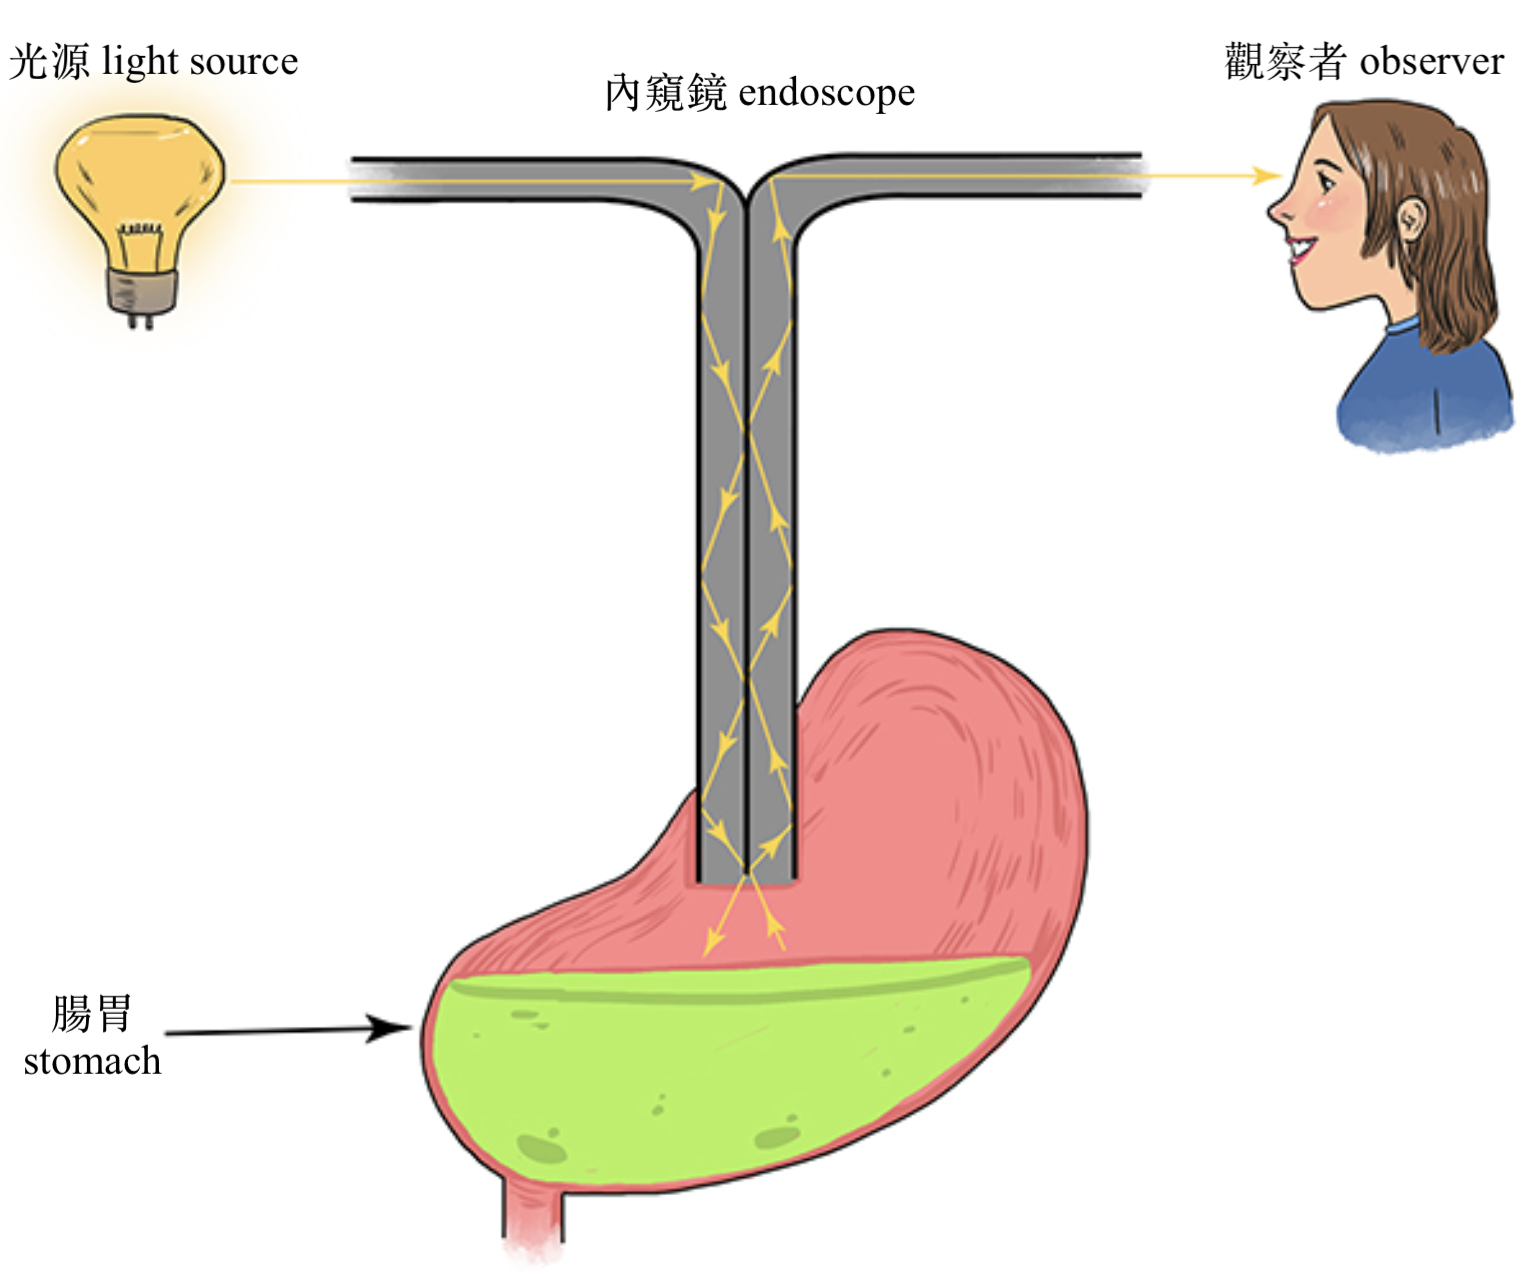
\includegraphics[width=.7\linewidth]{assets/d9j82323d3.png}
        \caption{光纖被用於對患者進行身體內部檢查。optical fiber is used for internal examination of the patient by doctors}
    \end{figure}
\end{frame}














































































\end{document}